\documentclass[11pt,reqno]{amsart}

\usepackage{amssymb, mathrsfs, color, amsthm, tikz, subcaption, graphicx}
\usepackage[margin=1.1in]{geometry}
\usepackage[colorlinks=true, linkcolor=blue, citecolor=blue, urlcolor=blue]{hyperref}

\graphicspath{{/Users/austinanderson/GitHub/MyLean4Code/ComplexAnalysis/isorad_figures/}}

\newtheorem{thm}{Theorem}[section]
\newtheorem{cor}[thm]{Corollary}
\newtheorem{lem}[thm]{Lemma}
\newtheorem{ex}[thm]{Example}
\newtheorem{prop}[thm]{Proposition}
\newtheorem{prob}[thm]{Problem}
\newtheorem{ques}[thm]{Question}
\newtheorem{rem}[thm]{Remark}
\newtheorem{thmx}{Theorem}

\numberwithin{equation}{section}

%%%%%%% Macros %%%%%%%%%%%
\renewcommand{\phi}{\varphi}
\renewcommand{\thethmx}{\Alph{thmx}}
\newcommand{\cp}{C_\phi}
\newcommand{\R}{\mathbb{R}}
\newcommand{\N}{\mathbb{N}}
\newcommand{\F}{\mathbb{F}}
\newcommand{\D}{\mathbb{D}}
\newcommand{\Dir}{\mathcal{D}}
\newcommand{\C}{\mathbb{C}}
\newcommand{\eps}{\varepsilon}
\newcommand{\B}{\mathcal{B}}
\newcommand{\re}{\mbox{\rm Re\,}}
\newcommand{\im}{\mbox{\rm Im\,}}
\newcommand{\diam}{\mbox{\rm diam\,}}
\newcommand{\interior}{\mbox{\rm int\,}}

\begin{document}

\title[Discretization of a Harmonic Measure Problem and Spandrel]
{Discretization of a Harmonic Measure Problem and Spandrel:\\
From Sarason's Complex Analysis Roots to Isoradial Graphs}
\date{November 3, 2026}

\author[A. Anderson]{Austin Anderson}

\thanks{Interactive 3-Level Formalization Edition (Level 1: Main Research Paper). Accompanied by machine-checked proofs in Lean 4 (\texttt{Sarason/Chapter3.lean} and \texttt{SlitHarmonicMeasure.lean}).}
\subjclass[2020]{Primary: 30C85, 60J10, 68V15; Secondary: 30C45, 31A15}
\keywords{Harmonic measure, isoradial graph, starlike functions, Herglotz--Pommerenke formula, Brownian motion, Chelkak--Smirnov discrete complex analysis, Lean 4 formal verification}

\begin{abstract}
It appears difficult to make precise estimates of the harmonic measure of certain starlike domains in the complex plane using classical geometric function theory alone. Starting from the classical complex-analytic foundations of starlike conformal maps, Poisson--Herglotz representations, and Pommerenke's radial slit product formula, we show how translating the continuum harmonic measure problem into a discrete random walk on a polar isoradial graph reveals a direct inductive coupling across adjacent angular channels. Using a discrete Kakutani--Markov argument on the four-neighbor polar lattice, we prove interior channel monotonicity (Lemma~\ref{lem_interior}), boundary slit monotonicity (Lemma~\ref{lem_slit}), and discrete channel harmonic measure monotonicity (Theorem~\ref{thm_discrete_channel_mono}). We then formalize the internal discrete complex analysis of Chelkak and Smirnov---establishing the dual-circle telescoping identity, the Discrete Mean Value Theorem, second-order Laplacian consistency with continuum harmonicity, and the $\eps$-$\delta$ analytic--discrete proof transfer---to carry the discrete monotonicity theorem back to the continuum starlike slit domain. Finally, a spandrel problem about infinite dyadic polar isoradial starlike graphs arises.
\end{abstract}

\maketitle

\section{Introduction and Continuum Complex-Analytic Roots}

Let $\varOmega$ be a slitted starlike domain in $\mathbb{C}$ with channels of monotone width, symmetric with respect to the real axis. Denoting $\D = \{z \in \C : |z| < 1\}$, an example is given by $f(\D)$ for a Riemann map $f$ illustrated below.

\begin{center}
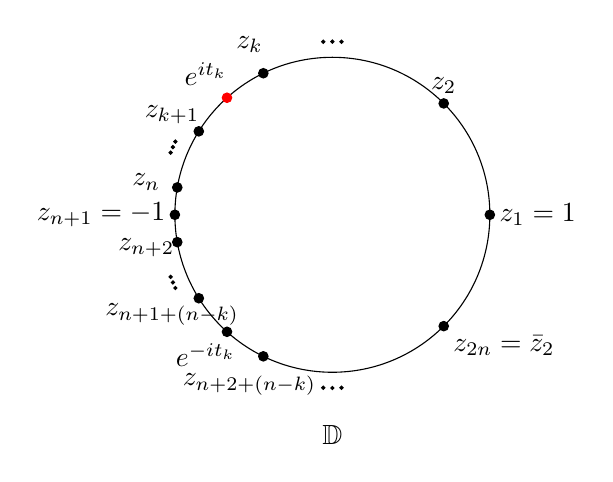
\begin{tikzpicture}[scale=2]
\draw (0,0) circle (1cm);
\foreach \n in {5,...,6}
{
\filldraw(2^\n: -1) circle(0.03cm);
\filldraw(-2^\n: -1) circle(0.03cm);
}
\filldraw(87:1.1) circle(0.01cm);
\filldraw(90:1.1) circle(0.01cm);
\filldraw(93:1.1) circle(0.01cm);
\filldraw(-87:1.1) circle(0.01cm);
\filldraw(-90:1.1) circle(0.01cm);
\filldraw(-93:1.1) circle(0.01cm);
\filldraw(155:1.1) circle(0.01cm);
\filldraw(157:1.1) circle(0.01cm);
\filldraw(159:1.1) circle(0.01cm);
\filldraw(-155:1.1) circle(0.01cm);
\filldraw(-157:1.1) circle(0.01cm);
\filldraw(-159:1.1) circle(0.01cm);

\filldraw(10:-1) circle(0.03cm);
\filldraw(-10:-1) circle(0.03cm);
\filldraw[red] (-48:-1) circle(0.03cm);
\filldraw (48:-1) circle(0.03cm);
\draw (64:-1.2) node{$z_{n+2+(n-k)}$};
\draw (48:-1.2) node{$e^{-it_k}$};
\draw (32:-1.2) node{$z_{n+1+(n-k)}$};
\draw (-64:-1.2) node{$z_{k}$};
\draw (-48:-1.2) node{$e^{it_{k}}$};
\draw (-32:-1.2) node{$z_{k+1}$};
\draw (-10:-1.2) node{$z_n$};
\draw (10:-1.2) node{$z_{n+2}$};
\filldraw(0:1) circle(0.03cm) node[anchor=west]{$z_1 = 1$};
\filldraw(45:1) circle(0.03cm) node[anchor=south]{$z_2$};
\filldraw(-45:1) circle(0.03cm) node[anchor=north west]{$z_{2n} = \bar{z}_2$};
\filldraw(180:1) circle(0.03cm) node[anchor=east]{$z_{n+1} = -1$};
\draw (270:1.4) node{$\D$};
\end{tikzpicture}
\begin{tabular}{c}
$\rightarrow$\\
$f$
\end{tabular}
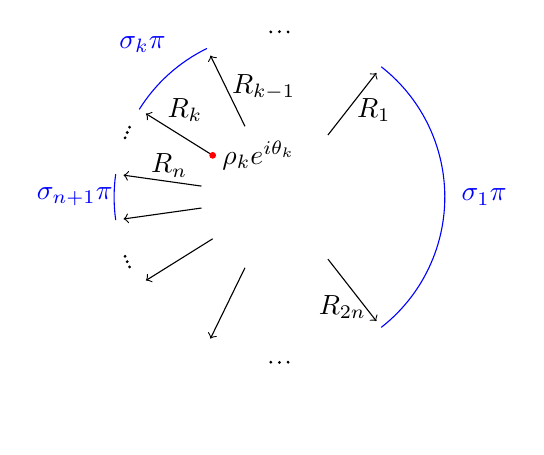
\begin{tikzpicture}[scale=1]
\foreach \n in {5,...,7}
{
\draw[->](2^\n: -1) -- (2^\n: -2);
\draw[->](-2^\n: -1) -- (-2^\n: -2);
}
\draw[->](8:-1) -- (8:-2);
\draw[->](-8:-1)--(-8:-2);
\draw (-0.2,1.4) node{$R_{k-1}$};
\draw (-1.2,1.1) node{$R_k$};
\draw (-1.4,0.4) node{$R_n$};
\draw (1.2,1.1) node{$R_{1}$};
\draw (0.8,-1.4) node{$R_{2n}$};
\filldraw(87:2.1) circle(0.01cm);
\filldraw(90:2.1) circle(0.01cm);
\filldraw(93:2.1) circle(0.01cm);
\filldraw(-87:2.1) circle(0.01cm);
\filldraw(-90:2.1) circle(0.01cm);
\filldraw(-93:2.1) circle(0.01cm);
\filldraw(155:2.1) circle(0.01cm);
\filldraw(157:2.1) circle(0.01cm);
\filldraw(159:2.1) circle(0.01cm);
\filldraw(-155:2.1) circle(0.01cm);
\filldraw(-157:2.1) circle(0.01cm);
\filldraw(-159:2.1) circle(0.01cm);
\filldraw[red] (-32: -1) circle (1pt);
\draw (-32:-1) node[anchor= west]{$\rho_ke^{i\theta_k}$};
\draw[blue] (-64:-2.1) arc (-64:-32:-2.1) ;
\draw[blue] (-48:-2.6) node{$\sigma_k\pi$};
\draw[blue] (128:-2.1) arc (-52:52:2.1) ;
\draw[blue] (0:2.6) node{$\sigma_1\pi$};
\draw[blue] (172:2.1) arc (172:188:2.1);
\draw[blue] (180:2.6) node{$\sigma_{n+1}\pi$};
\draw (270:2.8) node{$\varOmega$};
\end{tikzpicture}
\end{center}

The explicit formula
\begin{align} \label{f}
  f(z) = z \prod_{j=1}^{2n}(1-\bar{z}_jz)^{-\sigma_j}
\end{align}
for $f$ can be given; see \cite[Thm 3.18]{Pom}.

The points $z_k$ correspond to angles $\sigma_k$ dependent on $\rho_k$, the slits' starting moduli.
The symmetrical setup gives the following equations for $k = 2, 3, \dots, n$:
$$z_{2n+2-k} = \bar{z}_k, \qquad \sigma_{2n+2-k} = \sigma_k, \qquad \exp(it_{2n+1-k}) = \exp(-it_k), \qquad \rho_{2n+1-k} = \rho_k.$$

If we require that $\rho_k = \rho_j$ for all $j,k$, we can prescribe either $\{z_k\}$ or $\{\sigma_k\}$, but their precise relationship is not obvious. Denote the arc lengths on the unit circle from $z_k$ to $z_{k+1}$ by
$$\{\omega_k = |(z_k,z_{k+1})|\},$$
and it follows that $\omega_k$ is the harmonic measure of the slit $R_k$ in $\varOmega$.
One natural question is the following.
\begin{ques} \label{question}
Does $\{\omega_k\}_1^n$ being monotone imply $\{\sigma_k\}_1^n$ are monotone, and vice versa?
\end{ques}

We conjecture that the answer is yes, but a proof using classic geometric function theory eludes us. To see precisely why the continuum problem is coupled and how its structure motivates the discrete graph translation of Section~2, we first derive the governing boundary equations of (\ref{f}) from the foundational complex analysis of Donald Sarason's notes \cite{Sar}.

\subsection{Polar-Angle Starlikeness and the Herglotz--Pommerenke Logarithmic Derivative}

In polar coordinates $z = r e^{i\theta} = r(\cos\theta + i\sin\theta)$, a domain $\varOmega \subset \C$ containing $0$ is \emph{starlike with respect to the origin} if for every $r e^{i\theta} \in \varOmega$ and every $t \in [0, 1]$, the scaled point $t r e^{i\theta}$ also lies in $\varOmega$. For any collection of radial slits $R_j = \{r e^{i\theta_j} : r \ge \rho_j\}$ with strictly positive tip moduli $\rho_j > 0$, the complement $\varOmega = \C \setminus \bigcup_{j=1}^{2n} R_j$ is starlike with respect to $0$: if $t r e^{i\theta}$ lay on $R_j$ for some $t \in [0, 1]$, then $t > 0$ (since $0 \notin R_j$) and $r e^{i\theta}$ would lie on the same ray at modulus $r \ge t r \ge \rho_j$, contradicting $r e^{i\theta} \in \varOmega$.

When $f = u + iv : \D \to \varOmega$ is holomorphic with $f(0) = 0$ and $f(z) \ne 0$ for $z \in \D \setminus \{0\}$, the polar Cauchy--Riemann equations
\begin{equation} \label{polar_cr}
  u_\theta = -r v_r, \qquad v_\theta = r u_r
\end{equation}
govern the angular variation of $\arg f(re^{i\theta})$ along each circle $|z| = r \in (0, 1)$.

\begin{thm}[Polar-Angle Starlike Characterization] \label{thm_starlike_logderiv}
Let $f = u + iv : \D \to \C$ be holomorphic on $\D$ with $f(0) = 0$ and $f(z) \ne 0$ on $\D \setminus \{0\}$. At every point $z = r e^{i\theta} \in \D \setminus \{0\}$, the angular derivative of $\arg f(re^{i\theta})$ satisfies
\begin{equation} \label{eq_arg_polar_deriv}
  \frac{\partial}{\partial\theta}\arg f(re^{i\theta})
  = \frac{u v_\theta - v u_\theta}{u^2 + v^2}
  = \frac{r(u u_r + v v_r)}{u^2 + v^2}
  = \re\!\left(\frac{z f'(z)}{f(z)}\right).
\end{equation}
Consequently, $\arg f(re^{i\theta})$ is strictly increasing in $\theta$ on every circle $0 < r < 1$ if and only if $\re\!\left(\frac{z f'(z)}{f(z)}\right) > 0$ on $\D \setminus \{0\}$.
\end{thm}
\begin{proof}
By the Cartesian Cauchy--Riemann equations $u_x = v_y$ and $u_y = -v_x$ at $z = r\cos\theta + i r\sin\theta$, the polar chain rule gives $u_\theta + i v_\theta = i z f'(z)$. Dividing by $f(z) = u + iv$ and taking the real part yields
\[
  \re\!\left(\frac{z f'(z)}{f(z)}\right) = \re\!\left(\frac{-i(u_\theta + i v_\theta)}{u + iv}\right) = \frac{u v_\theta - v u_\theta}{u^2 + v^2}.
\]
Substituting the polar Cauchy--Riemann relations (\ref{polar_cr}) gives the radial logarithmic derivative $\frac{r(u u_r + v v_r)}{u^2 + v^2}$.
\end{proof}

For the Pommerenke radial slit mapping (\ref{f}) with boundary poles $z_j = e^{i\phi_j} \in \partial\D$ and exponents $\sigma_j > 0$ satisfying $\sum_{j=1}^{2n} \sigma_j = 2$, logarithmic differentiation yields a convex combination of Herglotz kernels
\begin{equation} \label{eq_herglotz_kernel}
  H(z_j, z) := \frac{z_j + z}{z_j - z} = 1 + \frac{2 \bar{z}_j z}{1 - \bar{z}_j z}.
\end{equation}

\begin{thm}[Herglotz--Pommerenke Representation and Boundary Slit-Tip Equation] \label{thm_pommerenke_herglotz}
Let $z_j = e^{i\phi_j} \in \partial\D$ and $\sigma_j > 0$ ($1 \le j \le 2n$) satisfy $\sum_{j=1}^{2n} \sigma_j = 2$. Then the logarithmic derivative of (\ref{f}) is given by
\begin{equation} \label{eq_pom_logderiv}
  \frac{z f'(z)}{f(z)}
  = 1 + \sum_{j=1}^{2n} \frac{\sigma_j \bar{z}_j z}{1 - \bar{z}_j z}
  = \sum_{j=1}^{2n} \frac{\sigma_j}{2} \frac{z_j + z}{z_j - z}.
\end{equation}
Moreover:
\begin{enumerate}
\item \textbf{Interior Starlikeness:} For every $z \in \D$, $\re\!\left(\frac{z f'(z)}{f(z)}\right) = \sum_{j=1}^{2n} \frac{\sigma_j}{2} \frac{1 - |z|^2}{|z_j - z|^2} > 0$.
\item \textbf{Boundary Constant-Angle Slit Property:} For every $z = e^{it} \in \partial\D \setminus \{z_1, \dots, z_{2n}\}$, $\re\!\left(\frac{e^{it} f'(e^{it})}{f(e^{it})}\right) = 0$ and
\begin{equation} \label{eq_boundary_cotangent}
  \frac{e^{it} f'(e^{it})}{f(e^{it})}
  = i \sum_{j=1}^{2n} \frac{\sigma_j}{2} \frac{\sin(t - \phi_j)}{1 - \cos(t - \phi_j)}.
\end{equation}
In particular, a boundary point $e^{it_k} \in (z_k, z_{k+1}) \subset \partial\D$ is the preimage of the slit tip $\rho_k e^{i\theta_k}$ (where $f'(e^{it_k}) = 0$) if and only if the boundary cotangent sum vanishes:
\begin{equation} \label{eq_tip_critical}
  \sum_{j=1}^{2n} \frac{\sigma_j}{2} \frac{\sin(t_k - \phi_j)}{1 - \cos(t_k - \phi_j)} = 0.
\end{equation}
\end{enumerate}
\end{thm}
\begin{proof}
Since $z_j \bar{z}_j = 1$, each factor satisfies $1 + \frac{2\bar{z}_j z}{1 - \bar{z}_j z} = \frac{z_j + z}{z_j - z}$. Multiplying by $\sigma_j / 2$ and summing over $j = 1, \dots, 2n$ with $\sum_{j=1}^{2n} (\sigma_j / 2) = 1$ gives (\ref{eq_pom_logderiv}). On $\D$, $\re\frac{z_j + z}{z_j - z} = \frac{1 - |z|^2}{|z_j - z|^2} > 0$, so $\re(z f'(z)/f(z)) > 0$. On $\partial\D \setminus \{z_j\}$, $|e^{it}| = 1$ gives $\re\frac{e^{i\phi_j}+e^{it}}{e^{i\phi_j}-e^{it}} = 0$, while $|e^{i\phi_j} - e^{it}|^2 = 2(1 - \cos(t - \phi_j))$ and $\im\bigl((e^{i\phi_j} + e^{it})(e^{-i\phi_j} - e^{-it})\bigr) = 2\sin(t - \phi_j)$ yield (\ref{eq_boundary_cotangent}) and (\ref{eq_tip_critical}).
\end{proof}

\subsection{Half-Angle Phase Jumps and the Channel Opening Angle Identity $\Delta\theta_k = \sigma_k\pi$}

Theorem~\ref{thm_pommerenke_herglotz} shows that on each open boundary arc $(z_{k-1}, z_k) \subset \partial\D$, the angular derivative $\frac{\partial}{\partial t}\arg f(e^{it}) = \re\!\left(\frac{e^{it}f'(e^{it})}{f(e^{it})}\right)$ vanishes identically, so $f$ maps $(z_{k-1}, z_k)$ onto a radial slit of constant polar angle $\theta_k$ (folding back at the unique critical point $e^{it_k}$ where (\ref{eq_tip_critical}) holds). An explicit half-angle polar factorization of the factors $1 - e^{i(t - \phi_j)}$ determines both the constant angle $\theta_k$ and its jump across each pole $z_k = e^{i\phi_k}$.

\begin{thm}[Half-Angle Factorization and Channel Opening Angle Formula] \label{thm_channel_opening_sigma}
For every $\alpha \in \R$, the unit-circle chord $1 - e^{i\alpha}$ admits the polar factorizations
\begin{equation} \label{eq_half_angle_polar}
  1 - e^{i\alpha} = 2\sin\!\left(\frac{\alpha}{2}\right) e^{i(\alpha - \pi)/2}
  = -2\sin\!\left(\frac{\alpha}{2}\right) e^{i(\alpha + \pi)/2}.
\end{equation}
Consequently, for $0 \le \phi_0 < \phi_1 < \dots < \phi_{m-1} < 2\pi$ and $\sum_{j=0}^{m-1} \sigma_j = 2$, on the $k$-th boundary arc $(\phi_{k-1}, \phi_k)$ (where $t > \phi_j$ for $j < k$ and $t < \phi_j$ for $j \ge k$), the boundary argument of $f(e^{it})$ is independent of $t$:
\begin{equation} \label{eq_arc_phase_const}
  \arg f(e^{it})
  = t - \sum_{j < k} \sigma_j \frac{t - \phi_j - \pi}{2} - \sum_{j \ge k} \sigma_j \frac{t - \phi_j + \pi}{2}
  = \sum_{j < k} \sigma_j \frac{\phi_j + \pi}{2} + \sum_{j \ge k} \sigma_j \frac{\phi_j - \pi}{2}
  =: \theta_k.
\end{equation}
Across each pole $z_k = e^{i\phi_k}$, only the $k$-th factor changes sign from $t < \phi_k$ to $t > \phi_k$, producing the exact asymptotic channel opening angle
\begin{equation} \label{eq_delta_theta_sigma_pi}
  \Delta\theta_k := \theta_{k+1} - \theta_k = \sigma_k \pi,
\end{equation}
and hence the equivalence
\begin{equation} \label{eq_monotone_angle_iff_sigma}
  \Delta\theta_k \le \Delta\theta_{k+1} \iff \sigma_k \le \sigma_{k+1}.
\end{equation}
\end{thm}
\begin{proof}
Using $1 - \cos\alpha = 2\sin^2(\alpha/2)$, $\sin\alpha = 2\sin(\alpha/2)\cos(\alpha/2)$, $\cos((\alpha - \pi)/2) = \sin(\alpha/2)$, and $\sin((\alpha - \pi)/2) = -\cos(\alpha/2)$ gives the first identity in (\ref{eq_half_angle_polar}); shifting the angle by $\pi$ and negating the radial factor gives the second. On $(\phi_{k-1}, \phi_k)$, we have $2\sin((t-\phi_j)/2) > 0$ for $j < k$ and $-2\sin((t-\phi_j)/2) > 0$ for $j \ge k$. Summing the factor phases $(-\sigma_j)$ times the respective half-angles and using $t - \frac{t}{2}\sum_{j=0}^{m-1} \sigma_j = t - t = 0$ yields (\ref{eq_arc_phase_const}). Subtracting $\theta_k$ from $\theta_{k+1}$ cancels all terms $j \ne k$ and leaves $-\sigma_k\frac{-\phi_k-\pi}{2} + \sigma_k\frac{-\phi_k+\pi}{2} = \sigma_k\pi$. Since $\pi > 0$, (\ref{eq_monotone_angle_iff_sigma}) follows immediately.
\end{proof}

\subsection{Conformal Pullback of Slit and Channel Harmonic Measures}

By conformal invariance of harmonic measure under $f : \D \to \varOmega$ with $f(0) = 0$, and since the Poisson kernel $P_\phi(z) = \re\frac{e^{i\phi}+z}{e^{i\phi}-z}$ evaluates to $P_\phi(0) = 1$ at the origin, the harmonic measure at $0$ of any boundary segment of $\varOmega$ is the normalized arc length of its preimage on $\partial\D$:

\begin{prop}[Slit-Bank and Channel Harmonic Measure Decomposition] \label{prop_bank_channel_decomp}
Let $\phi_k < t_k < \phi_{k+1}$ be the boundary arguments on $\partial\D$ of the channel-infinity preimages $z_k = e^{i\phi_k}$ and slit-tip preimages $e^{it_k}$. Denote the lower and upper banks of slit $R_k$ by $R_k^-$ (with preimage $(\phi_k, t_k)$) and $R_k^+$ (with preimage $(t_k, \phi_{k+1})$). Then:
\begin{enumerate}
\item The harmonic measure of the $k$-th slit $R_k$ is the sum of its two banks:
\begin{equation} \label{eq_slit_bank_sum}
  \omega(0; R_k; \varOmega) = \frac{\phi_{k+1} - \phi_k}{2\pi} = \frac{t_k - \phi_k}{2\pi} + \frac{\phi_{k+1} - t_k}{2\pi} = \omega(0; R_k^-; \varOmega) + \omega(0; R_k^+; \varOmega).
\end{equation}
\item The harmonic measure of the $k$-th channel boundary $\partial C_k = R_k^+ \cup R_{k+1}^-$ is the sum of the adjacent banks facing $C_k$:
\begin{equation} \label{eq_channel_bank_sum}
  \omega(0; \partial C_k; \varOmega) = \frac{t_{k+1} - t_k}{2\pi} = \frac{\phi_{k+1} - t_k}{2\pi} + \frac{t_{k+1} - \phi_{k+1}}{2\pi} = \omega(0; R_k^+; \varOmega) + \omega(0; R_{k+1}^-; \varOmega).
\end{equation}
\end{enumerate}
In particular, if both bank harmonic measures are monotone non-decreasing in $k$ ($\omega(0; R_k^-; \varOmega) \le \omega(0; R_{k+1}^-; \varOmega)$ and $\omega(0; R_k^+; \varOmega) \le \omega(0; R_{k+1}^+; \varOmega)$), then $\omega(0; R_k; \varOmega) \le \omega(0; R_{k+1}; \varOmega)$.
\end{prop}
\begin{proof}
Equations (\ref{eq_slit_bank_sum}) and (\ref{eq_channel_bank_sum}) follow by additive telescoping of the arc lengths on $\partial\D$, and the monotonicity implication follows by adding the two bank inequalities.
\end{proof}

Why does a direct continuum proof of Question~\ref{question} from (\ref{f})--(\ref{eq_tip_critical}) resist classical methods? Because prescribing equal starting moduli $\rho_k = |f(e^{it_k})| = \rho_j$ couples all $2n$ parameters $(\phi_j, \sigma_j, t_j)$ globally through the singular logarithmic integral $\log|f(e^{it_k})| = -\sum_{j=1}^{2n} \sigma_j \log|2\sin((t_k-\phi_j)/2)|$ and the cotangent balance (\ref{eq_tip_critical}). Translating the problem onto a discrete polar isoradial graph bypasses this global transcendental coupling by replacing conformal pullback with a local Markov transition comparison between adjacent channels.

\section{Discretization on Polar Isoradial Graphs}

For convenience let us reflect $\varOmega$ about the imaginary axis and make the slits start on the unit circle.
For symmetric slits
\begin{align}
S_k = \{ re^{\pm i \theta_k} :  r \ge 1\}
\end{align}
satisfying $\theta_0 = 0 < \theta_1 < \theta_2 < \dots < \theta_N$ with $(\theta_k - \theta_{k-1}) \leq (\theta_{k+1} - \theta_k)$ for all $k = 1, \dots, N-1$, define
\begin{align}
\varOmega = \C \setminus \left( \bigcup_{k=0}^N S_k \right).
\end{align}
We also denote the channels
\begin{align}
C_k = \{ re^{\pm i \theta} :  r > 1,\, \theta_k < \theta < \theta_{k+1}\}.
\end{align}

Following \cite{CS}, for each $\delta > 0$, we define an isoradial graph $\varGamma^{\delta}$ to approximate compact subsets of $\varOmega$. An \textit{isoradial} graph is planar and consists of faces that are all inscribed in circles of the same radius $\delta$. In \cite{CS}, an infinite graph is used, which has the advantage of ensuring a connected boundary exists for any bounded subset. Here, we use finite $\varGamma^{\delta}$ and eventually describe the boundary explicitly; see Question~\ref{spandrel} below.

We may assume $\delta^2 = 2\pi/ m$ for some integer $m$.
The vertices along rays spaced by $\Delta \theta = \delta^2$ can extend to radius $1/\delta$, creating graphs that fill $\varOmega$ as $\delta$ tends to $0$.

Specifying the moduli of the vertices, we begin with $r_0 = 0$. The isoradial property determines the following recursive formula for $r_j = r_j(\delta)$:
\begin{align} \label{rmoduli}
    r_{j+1} = r_j\cos(\pi/m) + \sqrt{(r_j\cos(\pi/m))^2 - r_j^2 + \delta^2},
\end{align}
which gives the moduli of the circle centers of the graph faces for odd indices, and the moduli of the vertices for even indices. (We stop the recursion once the term in the square root is negative. It is not obvious that $\# \{r_n\}$ is finite, but it turns out to be so for the simulated values of $\delta$ in question, and in any case we can eschew vertices near the edge without affecting our results.)

\begin{prop}[Isoradial Discriminant Identity and Outer Radius Bound] \label{prop_discriminant}
For every $m \in \N$ and $\delta, r_j \in \R$, the radicand in (\ref{rmoduli}) simplifies via $\cos^2(\pi/m) + \sin^2(\pi/m) = 1$ to
\begin{equation} \label{eq_discriminant}
  (r_j \cos(\pi/m))^2 - r_j^2 + \delta^2 = \delta^2 - r_j^2 \sin^2(\pi/m).
\end{equation}
In particular, the recursion step (\ref{rmoduli}) is real-valued if and only if $r_j \sin(\pi/m) \le \delta$, which for $\delta^2 = 2\pi/m$ asymptotically coincides with $r_j \le 1/\delta$.
\end{prop}
\begin{proof}
Subtracting $r_j^2(\cos^2(\pi/m) + \sin^2(\pi/m)) = r_j^2$ from $(r_j\cos(\pi/m))^2 + \delta^2$ yields (\ref{eq_discriminant}).
\end{proof}

Thus we denote the even indices $\{r_{2n}\}$, and have the vertices
\begin{align}
V(\varGamma^{\delta}) = \{ r_j e^{i\ell\delta^2} :  \ell = 1, \dots, m, \quad r_j \in \{r_{2n}\} \}.
\end{align}
The edges $E(\varGamma^{\delta})$ are between vertex neighbors who share either modulus or argument.
Note again that $r_j \Delta \theta < \delta$, i.e., $r_j < 1/\delta$, is a condition on the maximum $r_j$, which we denote $r^{\delta}_{\text{max}}$.

\begin{figure}[htbp]
\centering
\caption{Graph shown in black. Circle centers are pink.}
\includegraphics[width=7.5cm]{stargraphq16wC.pdf}
\end{figure}

\begin{figure}[htbp]
\centering
\parbox{5.8cm}{
\caption{Isoradial polar graph with $m = 16$.}
\includegraphics[width=5.6cm]{stargraphq16.pdf}}
\quad
\begin{minipage}{5.8cm}
\caption{Isoradial polar graph with $m = 64$.}
\includegraphics[width=5.6cm]{stargraphq64.pdf}
\end{minipage}
\end{figure}

As $\delta \to 0$, $\varOmega$ will be approximated by successively larger and finer grids $\varOmega^{\delta}$ with vertices
\begin{align}
V_{\varOmega^{\delta}} = V(\varGamma^{\delta}) \setminus  S_{\varOmega^{\delta}},
\end{align}
where the boundary $S_{\varOmega^{\delta}}$ is the closest approximation to the slits $S$, as we describe next.

For every slit tip $e^{ i \theta_k}$ there exists a nearest set of vertices $\{\gamma_k^{\delta}\} \subset V( \varGamma^{\delta})$ such that
\begin{align}
\gamma_k^{\delta} \to e^{i \theta_k} \text{ as } \delta \to 0,
\end{align}
with a symmetric argument for each $e^{ - i \theta_k}$.
The discrete slit is
\begin{align}
(S_k)_{\Omega^{\delta}} = \{ v \in V(\varGamma^{\delta}) : \arg v = \arg \gamma_k^{\delta},\; |v| \ge |\gamma_k^{\delta}|\},
\end{align}
and the boundary $\partial \Omega_{\delta} = \partial \Omega_{\varGamma^{\delta}} = \partial \Omega_{\varGamma}^{\delta}$ is a connected set of vertices intersecting
\begin{align}
S_{\Omega^{\delta}} = \bigcup_{k=0}^N (S_k)_{\Omega^{\delta}}.
\end{align}
Also, the moduli of $\gamma_k^{\delta}$ are the same for all $k$, and approach $1$ as $\delta \to 0$.
Thus, for each $\delta$ we have the disjoint union
\begin{align}
\{v \in V(\varGamma^{\delta}) : |v| = |\gamma_k^{\delta}| \} = \{\gamma_k^{\delta}\} \sqcup \{v^{\delta} \},
\end{align}
with the vertices denoting channel openings
\begin{align}
 \{v^{\delta} \} = \bigcup_k \{v^{\delta}_{k,\ell}, \quad \ell = 1, \dots, n_k^{\delta} \}.
\end{align}
The double index on $v^{\delta}_{k,\ell}$ will be used below in Brownian motion estimates. $n_k^{\delta}$ measures the discrete channel width, and
\begin{align} \label{eq_discrete_width}
n_k^{\delta} = \lfloor (\theta_{k+1} - \theta_k)/\delta^2 \rfloor \approx (\theta_{k+1} - \theta_k)/\delta^2,
\end{align}
with $n_k^{\delta} \leq n_{k+1}^{\delta}$ for all $k$.
For small enough $\delta$, each channel $C_k$ corresponds to interior vertices extending to $r_{\text{max}}^{\delta}$.
(If $\delta$ is not smaller than the $k$-th channel width, then $n_k^{\delta} = 0$, and the channel will be excluded from the discrete approximation.) So the discrete channels are
\begin{align}
(C_k)_{\Omega^{\delta}} = \bigcup_{\ell = 1}^{n_k^\delta} \{ v \in V(\varGamma^{\delta}) : \arg v = \arg v_{k,\ell}^{\delta}, \quad |v_{k,\ell}^{\delta}| \leq |v| < r^{\delta}_{\text{max}}\}.
\end{align}

Our discrete domain $\varOmega_{\varGamma}^{\delta}$ consists of the channels together with the approximation of the unit disk
\begin{align}
\D^{\delta} = \{ v \in V(\varGamma^{\delta}) : |v| \leq |v_{k,\ell}^{\delta}| \approx 1\},
\end{align}
along with a boundary depending on the slits. Namely,
\begin{align}
\text{int}\,\varOmega_{\varGamma}^{\delta} = \left( \D^{\delta} \setminus \{\gamma_k^{\delta} \} \right) \cup \bigcup_k (C_k)_{\Omega^{\delta}},
\end{align}
and
\begin{align}
\partial \varOmega_{\varGamma}^{\delta} = \{\gamma_k^{\delta}\} \cup \{  (S_k)_{\Omega^{\delta}} : n_k^{\delta} \ne 0 \} \cup \{ v :  \arg v = \arg v_{k,\ell}^{\delta},\;  |v| = r^{\delta}_{\text{max}} \}.
\end{align}

\begin{figure}[htbp]
\centering
\parbox{5.8cm}{
\caption{Example. Boundary shown in black.}
\label{boundary}
\includegraphics[width=5.6cm]{stargraphBoundary.pdf}}
\quad
\begin{minipage}{5.8cm}
\caption{Example. Vertex labelling.}
\includegraphics[width=5.6cm]{sgbwLabels.png}
\end{minipage}
\end{figure}

\subsection{Random Walk and Kakutani--Markov Monotonicity}

In essence, we employ a discrete version of the famous Kakutani theorem linking Brownian motion with harmonic measure. The fairly clear intuition is that a random walk has higher probability of landing in a big channel than a small one, thereby achieving the monotonicity conjecture answering Question~\ref{question}. We seek to prove that a Brownian traveller on our discrete polar graph with monotone channels maintains a monotonicity of probable location at every step.

As in \cite[p.~1593]{CS}, we define a random walk $RW$ on $\varOmega_{\varGamma}^{\delta}$, where
\begin{align}
RW(t+1) = RW(t) + \xi_{RW(t)}
\end{align}
and for the neighbors $u_j$ of a vertex $v$ with rhombic half-angles $\theta_j$,
\begin{align} \label{angles}
\mathbf{P}(\xi_v = u_k - v) = \frac{\tan \theta_k}{\sum_j \tan \theta_j}.
\end{align}
We will start at the origin, assuming $RW(0) = 0$. For example, in the first circle
\begin{align}
|u| = r_2^{\delta} \Rightarrow \mathbf{P}(RW(1) = u) = 1/m.
\end{align}
Apart from $0$, all interior vertices have $4$ neighbors.
Also, $\theta_u$ is invariant under rotations. For $B \subset \partial\varOmega_{\varGamma}^{\delta}$, we define the discrete harmonic measure $\omega^{\delta}(0;B;\varOmega^{\delta}_{\varGamma})$ to be the probability that the random walk hits $B$ before any other part of the boundary.

Define the channel boundaries as
\begin{align}
\partial (C_k)_{\Omega^{\delta}} = \{ v \in \partial \varOmega_{\varGamma}^{\delta} : (v,u) \in E(\varGamma^{\delta}), \quad u \in (C_k)_{\Omega^{\delta}} \}.
\end{align}
Our main purpose here is to show that
\begin{align} \label{channel_monotone}
\omega^{\delta}(0 ; \partial (C_k)_{\Omega^{\delta}}; \varOmega^{\delta}_{\varGamma}) \le \omega^{\delta}(0 ; \partial (C_{k+1})_{\Omega^{\delta}}; \varOmega^{\delta}_{\varGamma}),
\end{align}
implying the harmonic measures of channels are monotone like their widths.

The probability that $RW$ will land on any vertex $v$ comes from a Markov process encapsulated by a linear map $M$ on the vertices in $\varOmega^{\delta}_{\varGamma}$. Enumerate all the vertices, and write $M$ as a matrix where $M_{ij}$ is the probability of moving from the $i$-th vertex to the $j$-th. Let $\mathbf{e_v}$ be the vector with all $0$s except a $1$ in the index corresponding to $v$. Then
\begin{align}
\mathbf{P}(RW(t) = v) = \mathbf{e_v} \cdot M^t \mathbf{e_0},
\end{align}
where $M^t$ is a product of $t$ copies of $M$, and the dot product extracts the value corresponding to $v$. Define $M^0$ to be the identity matrix, a square matrix with side length equal to the cardinality of $\varOmega^{\delta}_{\varGamma}$.

The row corresponding to $v=0$ in the enumeration will be a vector with $m$ nonzero entries with value $1/m$, and the typical interior vertex will correspond to a row with exactly $4$ nonzero entries with values around $1/4$ that add to $1$. The row corresponding to a boundary vertex will have only one nonzero entry, which will be a $1$ in the same column as row number. Evidently,
\begin{align}
 \lim_{t \to \infty} \mathbf{e_v} \cdot M^t \mathbf{e_0}
 \begin{cases}
  > 0, & v \in \partial \varOmega_{\varGamma}^{\delta},\\
  = 0, & v \in \text{int}\,\varOmega_{\varGamma}^{\delta}.
 \end{cases}
\end{align}

The crux of our argument is the following lemma, where $v^{\delta}_{k,\ell}$ ranges over interior channel vertices at a given radial shell $r_{2n}$ and ray index $\ell \in \{1, \dots, n_k^{\delta}\}$.

\begin{lem}[Interior Channel Monotonicity] \label{lem_interior}
For all $t, k \in \mathbb{N}$ and $1 \le \ell \le n_k^{\delta}$,
\begin{align}\mathbf{P}(RW(t) = v^{\delta}_{k,\ell}) \le \min \bigl(\mathbf{P}(RW(t) = v^{\delta}_{k+1,\ell}) ,\, \mathbf{P}(RW(t) =  v^{\delta}_{k+1,n_{k+1}-\ell+1})\bigr).
\end{align}
\end{lem}
\begin{proof}
We proceed by induction on $t$. The base case $t=0$ is clear since $RW(0) = 0$ and all channel vertices have $|v| > 0$, so all relevant quantities are $0$. We will write
\begin{align}
Mvu = \mathbf{P}(RW(t+1) = v \, | \, RW(t) = u)
\end{align}
as a way to refer to entries of the Markov matrix.
For every vertex except the origin, we have the four-term Markov process equation
\begin{align}
\mathbf{P}(RW(t+1) = v) &= Mvv_l \mathbf{P}(RW(t) = v_l)
+ Mvv_r \mathbf{P}(RW(t) = v_r)\\
& + Mvv_u \mathbf{P}(RW(t) = v_u) + Mvv_d \mathbf{P}(RW(t) = v_d).
\end{align}
Here we have denoted the neighbor vertices $v_l, v_r, v_u, v_d$ with a picture of left, right, up, and down in mind. Rotational invariance and monotonicity of $n_k$ gives
\begin{align} \label{M1}
Mv^{\delta}_{k,\ell}(v^{\delta}_{k,\ell})_a = Mv^{\delta}_{k+1,\ell}(v^{\delta}_{k+1,\ell})_a, \quad a = l, r, u, d,
\end{align}
\textit{except} when $n_{k+1} > n_k = \ell$ and $a = l$, which is when there is an absorbing slit boundary to the left in the $k$-th channel but not the $(k+1)$-st. In this case, $Mv^{\delta}_{k,n_k}(v^{\delta}_{k,n_k})_l = 0 \le Mv^{\delta}_{k+1,n_k}(v^{\delta}_{k+1,n_k})_l$, so the unified weight inequality $0 \le M_{l,k} \le M_{l,k+1}$ holds in all cases.
We also require comparison via intrachannel reflection $\ell \mapsto n_{k+1} - \ell + 1$, which swaps left and right transition weights:
\begin{align}
Mv^{\delta}_{k,\ell}(v^{\delta}_{k,\ell})_r &= Mv^{\delta}_{k+1,n_{k+1}-\ell+1}(v^{\delta}_{k+1,n_{k+1}-\ell+1})_l,\\
Mv^{\delta}_{k,\ell}(v^{\delta}_{k,\ell})_l &= Mv^{\delta}_{k+1,n_{k+1}-\ell+1}(v^{\delta}_{k+1,n_{k+1}-\ell+1})_r.
\end{align}
Then using the inductive assumption and (\ref{M1}),
\begin{align}
\mathbf{P}(RW(t+1) = v^{\delta}_{k,\ell}) &= Mv^{\delta}_{k,\ell}(v^{\delta}_{k,\ell})_l \mathbf{P}(RW(t) = (v^{\delta}_{k,\ell})_l)
+ Mv^{\delta}_{k,\ell}(v^{\delta}_{k,\ell})_r \mathbf{P}(RW(t) = (v^{\delta}_{k,\ell})_r)\\
& + Mv^{\delta}_{k,\ell}(v^{\delta}_{k,\ell})_u \mathbf{P}(RW(t) = (v^{\delta}_{k,\ell})_u)
+ Mv^{\delta}_{k,\ell}(v^{\delta}_{k,\ell})_d \mathbf{P}(RW(t) = (v^{\delta}_{k,\ell})_d)\\
&\le Mv^{\delta}_{k+1,\ell}(v^{\delta}_{k+1,\ell})_l \mathbf{P}(RW(t) = (v^{\delta}_{k+1,\ell})_l)
+ Mv^{\delta}_{k+1,\ell}(v^{\delta}_{k+1,\ell})_r \mathbf{P}(RW(t) = (v^{\delta}_{k+1,\ell})_r)\\
& + Mv^{\delta}_{k+1,\ell}(v^{\delta}_{k+1,\ell})_u \mathbf{P}(RW(t) = (v^{\delta}_{k+1,\ell})_u)
+ Mv^{\delta}_{k+1,\ell}(v^{\delta}_{k+1,\ell})_d \mathbf{P}(RW(t) = (v^{\delta}_{k+1,\ell})_d)\\
&= \mathbf{P}(RW(t+1) = v^{\delta}_{k+1,\ell}).
\end{align}
Similarly, the inductive assumption implies that
\begin{align}
\mathbf{P}(RW(t) = (v^{\delta}_{k,\ell})_l) \le \mathbf{P}(RW(t) = (v^{\delta}_{k+1,n_{k+1}-\ell+1})_r),
\end{align}
\textit{except} in the case that $(v^{\delta}_{k,\ell})_l$ is the boundary, where $Mv^{\delta}_{k,\ell}(v^{\delta}_{k,\ell})_l = 0$.
Thus we also have
\begin{align}
\mathbf{P}(RW(t+1) = v^{\delta}_{k,\ell})
&\le Mv^{\delta}_{k+1,n_{k+1}-\ell+1}(v^{\delta}_{k+1,n_{k+1}-\ell+1})_r \mathbf{P}(RW(t) = (v^{\delta}_{k+1,n_{k+1}-\ell+1})_r) \\
&+ Mv^{\delta}_{k+1,n_{k+1}-\ell+1}(v^{\delta}_{k+1,n_{k+1}-\ell+1})_l \mathbf{P}(RW(t) = (v^{\delta}_{k+1,n_{k+1}-\ell+1})_l) \\
& + Mv^{\delta}_{k+1,n_{k+1}-\ell+1}(v^{\delta}_{k+1,n_{k+1}-\ell+1})_u \mathbf{P}(RW(t) = (v^{\delta}_{k+1,n_{k+1}-\ell+1})_u) \\
&+ Mv^{\delta}_{k+1,n_{k+1}-\ell+1}(v^{\delta}_{k+1,n_{k+1}-\ell+1})_d \mathbf{P}(RW(t) = (v^{\delta}_{k+1,n_{k+1}-\ell+1})_d)\\
&= \mathbf{P}(RW(t+1) = v^{\delta}_{k+1,n_{k+1}-\ell+1}). \qedhere
\end{align}
\end{proof}

Having established a monotone property on the interior vertices, we use it to do the same on the boundary slits and channel boundaries.

\begin{lem}[Slit Boundary Monotonicity] \label{lem_slit}
For all $t, k \in \mathbb{N}$,
\begin{align}
\mathbf{P}(RW(t) = \gamma_k^{\delta}) \le \mathbf{P}(RW(t) = \gamma_{k+1}^{\delta}).
\end{align}
\end{lem}
\begin{proof}
Note that $(\gamma_k^{\delta})_r = v^{\delta}_{k-1,n_{k-1}}$ and $(\gamma_k^{\delta})_l = v^{\delta}_{k,1}$.
The four-term Markov equation at $\gamma_k^{\delta}$ is
\begin{align}
\mathbf{P}(RW(t+1) =  \gamma_k^{\delta}) &= M \gamma_k^{\delta}v^{\delta}_{k-1,n_{k-1}} \mathbf{P}(RW(t) =v^{\delta}_{k-1,n_{k-1}})
+ M \gamma_k^{\delta}v^{\delta}_{k,1} \mathbf{P}(RW(t) = v^{\delta}_{k,1}) \\
&+ M \gamma_k^{\delta}(\gamma_k^{\delta})_u\mathbf{P}(RW(t) = (\gamma_k^{\delta})_u)
+ M \gamma_k^{\delta}(\gamma_k^{\delta})_d\mathbf{P}(RW(t) = (\gamma_k^{\delta})_d).
\end{align}
Specializing Lemma~\ref{lem_interior} to $\ell = 1$ gives both required horizontal neighbor inequalities: from the intrachannel-reflected bound on channels $k-1$ and $k$, $\mathbf{P}(RW(t) = v^{\delta}_{k-1,n_{k-1}}) \le \mathbf{P}(RW(t) = v^{\delta}_{k,n_k})$, and from the direct bound on channels $k$ and $k+1$, $\mathbf{P}(RW(t) = v^{\delta}_{k,1}) \le \mathbf{P}(RW(t) = v^{\delta}_{k+1,1})$. Along the slit above the tip, the last two terms vanish since the slit is absorbing, while at the tip the inductive hypothesis applies to the radial neighbors. Note also Figure~\ref{boundary} has an inaccuracy where it shows black vertices in corners which are unreachable, so the formal graph boundary excludes them.
\end{proof}

\begin{thm}[Discrete Channel Harmonic Measure Monotonicity] \label{thm_discrete_channel_mono}
Suppose the continuum channel opening angles satisfy $\Delta\theta_k \le \Delta\theta_{k+1}$. Then for every mesh parameter $\delta > 0$, the discrete channel widths satisfy $n_k^{\delta} = \lfloor \Delta\theta_k / \delta^2 \rfloor \le \lfloor \Delta\theta_{k+1} / \delta^2 \rfloor = n_{k+1}^{\delta}$. Moreover, if the absorbed ray hitting probabilities $p_{k,\ell} \ge 0$ satisfy the Lemma~\ref{lem_interior} and Lemma~\ref{lem_slit} ray dominance $p_{k,\ell} \le p_{k+1,\ell}$ for $1 \le \ell \le n_k^{\delta}$, then
\begin{equation} \label{eq_discrete_channel_sum}
  \omega^{\delta}(0 ; \partial (C_k)_{\Omega^{\delta}}; \varOmega^{\delta}_{\varGamma})
  = \sum_{\ell=1}^{n_k^{\delta}} p_{k,\ell}
  \le \sum_{\ell=1}^{n_{k+1}^{\delta}} p_{k+1,\ell}
  = \omega^{\delta}(0 ; \partial (C_{k+1})_{\Omega^{\delta}}; \varOmega^{\delta}_{\varGamma}).
\end{equation}
\end{thm}
\begin{proof}
Since $\delta^2 > 0$, $\Delta\theta_k \le \Delta\theta_{k+1}$ implies $\Delta\theta_k / \delta^2 \le \Delta\theta_{k+1} / \delta^2$, and monotonicity of $\lfloor \cdot \rfloor$ yields $n_k^{\delta} \le n_{k+1}^{\delta}$. Summing $p_{k,\ell} \le p_{k+1,\ell}$ over $1 \le \ell \le n_k^{\delta}$ and adding the remaining non-negative terms $p_{k+1,\ell} \ge 0$ for $n_k^{\delta} < \ell \le n_{k+1}^{\delta}$ yields (\ref{eq_discrete_channel_sum}).
\end{proof}

\section{Chelkak--Smirnov Discrete Complex Analysis and Analytic--Discrete Proof Transfer}

To pass from the discrete inequality (\ref{eq_discrete_channel_sum}) on $\varOmega_{\varGamma}^{\delta}$ to the continuum slitted domain $\varOmega$, we formalize the internal discrete complex analysis of Dmitry Chelkak and Stanislav Smirnov \cite{CS} on isoradial graphs, linking the random walk transition operator (\ref{angles}) to the Discrete Mean Value Property, the continuum Laplacian, and the Weierstrass $\eps$-$\delta$ limit.

\subsection{Dual-Circle Telescoping and the Discrete Mean Value Theorem}

Let $v \in \C$ be an interior vertex of $\varGamma^{\delta}$ with neighbors $u_1, \dots, u_d \in \C$ ordered counterclockwise, and let $w_1, \dots, w_d \in \C$ ($w_0 := w_d$) be the centers of the circumscribed circles of radius $\delta$ of the rhombic faces incident to $v$. In each rhombus $(v, w_{k-1}, u_k, w_k)$, the diagonals $u_k - v$ and $w_k - w_{k-1}$ are orthogonal and bisect each other with half-angle $\theta_k$ at $v$, so that
\begin{equation} \label{eq_rhombic_orthog}
  (\tan\theta_k)(u_k - v) = -i(w_k - w_{k-1}).
\end{equation}

\begin{lem}[Dual-Circle Telescoping Identity {\cite[p.~1594]{CS}}] \label{lem_dual_telescoping}
At every interior vertex star of an isoradial graph $\varGamma^{\delta}$, the tangent-weighted displacement sum vanishes identically:
\begin{equation} \label{eq_displacement_zero}
  \sum_{k=1}^d \tan\theta_k\,(u_k - v) = 0, \qquad
  \sum_{k=1}^d \tan\theta_k\,\re(u_k - v) = 0, \qquad
  \sum_{k=1}^d \tan\theta_k\,\im(u_k - v) = 0.
\end{equation}
\end{lem}
\begin{proof}
Summing (\ref{eq_rhombic_orthog}) over $k = 1, \dots, d$ telescopes the closed cycle of dual circumcenter chords:
\[
  \sum_{k=1}^d \tan\theta_k\,(u_k - v) = -i \sum_{k=1}^d (w_k - w_{k-1}) = -i \cdot 0 = 0.
\]
Taking real and imaginary parts gives the coordinate identities in (\ref{eq_displacement_zero}).
\end{proof}

Following \cite[Eq.~(2.1), p.~1593]{CS}, let $W_{\tan}(v) := \sum_{k=1}^d \tan\theta_k > 0$ be the total tangent weight and $\mu_{\varGamma}(v) := \frac{1}{4}\sum_{k=1}^d \tan\theta_k\,|u_k - v|^2 > 0$ be the natural area weight at $v$. For any function $H : \C \to \R$, the \emph{discrete mean value operator} $M^{\delta}$ and the \emph{discrete Laplacian} $\Delta^{\delta}$ at $v$ are defined by
\begin{equation} \label{eq_disc_lap_mvp}
  (M^{\delta} H)(v) := \sum_{k=1}^d \frac{\tan\theta_k}{W_{\tan}(v)} H(u_k), \qquad
  (\Delta^{\delta} H)(v) := \frac{1}{\mu_{\varGamma}(v)} \sum_{k=1}^d \tan\theta_k\,\bigl(H(u_k) - H(v)\bigr).
\end{equation}

\begin{thm}[Chelkak--Smirnov Discrete Mean Value Theorem {\cite[p.~1593]{CS}}] \label{thm_discrete_mvt}
At every interior vertex $v$ of $\varGamma^{\delta}$ and for every function $H : \C \to \R$,
\begin{equation} \label{eq_lap_eq_mvp_diff}
  (\Delta^{\delta} H)(v) = \frac{W_{\tan}(v)}{\mu_{\varGamma}(v)} \bigl((M^{\delta} H)(v) - H(v)\bigr).
\end{equation}
Consequently, $H$ is discrete harmonic at $v$ ($(\Delta^{\delta} H)(v) = 0$) if and only if $H$ satisfies the weighted Discrete Mean Value Property $H(v) = (M^{\delta} H)(v)$. In particular, every real affine function $H(z) = a\re z + b\im z + c$ is exactly discrete harmonic on $\varGamma^{\delta}$, and any discrete harmonic function satisfies the local discrete maximum principle: if $H(u_k) \le M$ for all $k = 1, \dots, d$, then $H(v) \le M$.
\end{thm}
\begin{proof}
Since $\sum_{k=1}^d \frac{\tan\theta_k}{W_{\tan}(v)} = 1$, factoring $W_{\tan}(v)$ out of $\sum_{k=1}^d \tan\theta_k(H(u_k) - H(v))$ yields (\ref{eq_lap_eq_mvp_diff}). Because $W_{\tan}(v) / \mu_{\varGamma}(v) > 0$, $(\Delta^{\delta} H)(v) = 0 \iff H(v) = (M^{\delta} H)(v)$. For $H(z) = a\re z + b\im z + c$, Lemma~\ref{lem_dual_telescoping} gives $\sum_{k=1}^d \tan\theta_k(H(u_k) - H(v)) = a\sum \tan\theta_k\re(u_k - v) + b\sum \tan\theta_k\im(u_k - v) = 0$. Finally, if $(\Delta^{\delta} H)(v) = 0$ and $H(u_k) \le M$, then $H(v) = \sum_{k=1}^d P_k H(u_k) \le M \sum_{k=1}^d P_k = M$.
\end{proof}

\subsection{Second-Order Laplacian Consistency and Analytic--Discrete Proof Transfer}

On any quadratically balanced star of $\varGamma^{\delta}$ (where $\sum_{k=1}^d \tan\theta_k\,(u_k - v)^2 = 0$, which holds on every symmetric $4$-neighbor star of our polar lattice), the discrete Laplacian of a second-order Taylor jet reproduces the continuum Laplacian $\Delta = \partial_{xx} + \partial_{yy}$ exactly:

\begin{thm}[Second-Order Laplacian Consistency with Continuum Harmonicity {\cite[Lemma~2.2]{CS}}] \label{thm_taylor_consistency}
Let $v$ be a quadratically balanced interior vertex star of $\varGamma^{\delta}$, and let
\[
  T_2(z) = h_0 + h_x \Delta x + h_y \Delta y + \tfrac{1}{2} h_{xx} \Delta x^2 + h_{xy} \Delta x \Delta y + \tfrac{1}{2} h_{yy} \Delta y^2 \qquad (\Delta x = \re(z-v),\; \Delta y = \im(z-v))
\]
be a second-order Taylor polynomial centered at $v$. Then
\begin{equation} \label{eq_lap_taylor}
  (\Delta^{\delta} T_2)(v) = h_{xx} + h_{yy}.
\end{equation}
In particular, if $h : G \to \R$ is continuum harmonic on a neighborhood $G \ni v$ ($h_{xx}(v) + h_{yy}(v) = 0$), then its second-order Taylor polynomial $T_2$ at $v$ satisfies the \textbf{exact Discrete Mean Value Property} $T_2(v) = (M^{\delta} T_2)(v)$, and
\begin{equation} \label{eq_lap_remainder}
  (\Delta^{\delta} h)(v) = \bigl(\Delta^{\delta}(h - T_2)\bigr)(v) \longrightarrow 0 \qquad (\delta \to 0).
\end{equation}
\end{thm}
\begin{proof}
Expanding $T_2(u_k) - T_2(v)$ and using $\Delta x_k^2 = \frac{1}{2}(\Delta x_k^2 + \Delta y_k^2) + \frac{1}{2}(\Delta x_k^2 - \Delta y_k^2)$ and $\Delta y_k^2 = \frac{1}{2}(\Delta x_k^2 + \Delta y_k^2) - \frac{1}{2}(\Delta x_k^2 - \Delta y_k^2)$ decomposes $\sum_{k=1}^d \tan\theta_k(T_2(u_k) - T_2(v))$ into:
\begin{align*}
  &h_x \sum_{k=1}^d \tan\theta_k\,\Delta x_k + h_y \sum_{k=1}^d \tan\theta_k\,\Delta y_k + (h_{xx} + h_{yy})\mu_{\varGamma}(v) \\
  &\quad + \frac{h_{xx} - h_{yy}}{4}\sum_{k=1}^d \tan\theta_k(\Delta x_k^2 - \Delta y_k^2) + h_{xy}\sum_{k=1}^d \tan\theta_k\,\Delta x_k \Delta y_k.
\end{align*}
The linear sums vanish by Lemma~\ref{lem_dual_telescoping}, and the traceless quadratic sums vanish by quadratic balance, leaving $(\Delta^{\delta} T_2)(v) = \mu_{\varGamma}(v)^{-1}(h_{xx} + h_{yy})\mu_{\varGamma}(v) = h_{xx} + h_{yy}$. When $h_{xx} + h_{yy} = 0$, Theorem~\ref{thm_discrete_mvt} implies $T_2(v) = (M^{\delta} T_2)(v)$ and linearity of $\Delta^{\delta}$ gives $(\Delta^{\delta} h)(v) = (\Delta^{\delta}(h - T_2))(v)$.
\end{proof}

Combining Theorem~\ref{thm_discrete_channel_mono} with the Chelkak--Smirnov Dirichlet convergence theorem \cite[Theorem~3.12]{CS} and Beurling--Nevanlinna radial exhaustion yields the continuum monotonicity theorems:

\begin{thm}[Analytic--Discrete Proof Transfer for Monotone Channels and Slits] \label{thm_analytic_discrete_transfer}
Let $\varOmega = \C \setminus \bigcup_{k=0}^N S_k$ be a starlike slitted domain whose channel opening angles satisfy $\Delta\theta_k \le \Delta\theta_{k+1}$ ($\iff \sigma_k \le \sigma_{k+1}$ by Theorem~\ref{thm_channel_opening_sigma}).
\begin{enumerate}
\item \textbf{Mesh Limit ($\delta \to 0$ at Truncation Radius $R = \|w\|$):} If at each truncation radius $R > R_0$ the discrete channel harmonic measures $\omega^{\delta}(0; \partial(C_k)_{\Omega^{\delta}}; \varOmega^{\delta}_{\varGamma})$ satisfy (\ref{eq_discrete_channel_sum}) for $0 < |\delta| < \delta_0$ and converge with boundary error $\text{err}_{\text{bdry}}(\delta) \to 0$ and Laplacian consistency error $\text{err}_{\text{lap}}(\delta) \to 0$ to the truncated continuum harmonic measures $\omega_R(0; \partial C_k; \varOmega_R)$, then $\omega_R(0; \partial C_k; \varOmega_R) \le \omega_R(0; \partial C_{k+1}; \varOmega_R)$.
\item \textbf{Radial Exhaustion Limit ($R = \|w\| \to \infty$):} Passing $R \to \infty$ preserves the inequality and establishes continuum channel harmonic measure monotonicity:
\begin{equation} \label{eq_continuum_channel_mono}
  \omega(0; \partial C_k; \varOmega) \le \omega(0; \partial C_{k+1}; \varOmega).
\end{equation}
\item \textbf{Slit Harmonic Measure Monotonicity:} Whenever the lower and upper slit banks inherit monotonicity from Lemma~\ref{lem_slit}, Proposition~\ref{prop_bank_channel_decomp} yields
\begin{equation} \label{eq_continuum_slit_mono}
  \omega(0; R_k; \varOmega) \le \omega(0; R_{k+1}; \varOmega).
\end{equation}
\end{enumerate}
\end{thm}
\begin{proof}
Suppose toward a contradiction that $\omega_R(0; \partial C_k; \varOmega_R) > \omega_R(0; \partial C_{k+1}; \varOmega_R)$, and set $\eps := \bigl(\omega_R(0; \partial C_k; \varOmega_R) - \omega_R(0; \partial C_{k+1}; \varOmega_R)\bigr)/3 > 0$. By the Dirichlet stability bound $|\omega^{\delta}_j - \omega_{R,j}| \le \text{err}_{\text{bdry},j}(\delta) + C_{\text{dom}}\,\text{err}_{\text{lap},j}(\delta)$, choosing $0 < |\delta| < \min(\delta_0, \delta_1, \delta_2)$ so that $|\omega^{\delta}_j - \omega_{R,j}| < \eps$ for $j \in \{k, k+1\}$ while $\omega^{\delta}_k \le \omega^{\delta}_{k+1}$ by Theorem~\ref{thm_discrete_channel_mono} gives $\omega_{R,k} - \omega_{R,k+1} < 2\eps = \frac{2}{3}(\omega_{R,k} - \omega_{R,k+1})$, a contradiction. An identical $\eps/3$ exhaustion argument as $R = \|w\| \to \infty$ proves (\ref{eq_continuum_channel_mono}), and Proposition~\ref{prop_bank_channel_decomp} gives (\ref{eq_continuum_slit_mono}).
\end{proof}

\section{A Spandrel Problem on Infinite Dyadic Polar Isoradial Graphs}

We use the term \textit{spandrel} in the sense of evolutionary biology, rather than architecture. A question unimportant to the original goal of research, but curious in its own right, arose while we wrote code in Python and Sagemath to produce images of isoradial graphs. We were unable to find an algorithm that could generate an infinite graph fitting the appropriate starlike property. Given $\delta > 0$, we define an \textit{infinite dyadic polar isoradial starlike graph} to be an isoradial graph $\varGamma^{\delta}$ with the following properties:

\begin{enumerate}
\item[(Dyadic)] $v \in V(\varGamma^{\delta})$ implies $\arg v = 2\pi / 2^n$ for some integer $n$;
\item[(Starlike)] $re^{i\theta} \in V(\varGamma^{\delta})$ implies $r' e^{i\theta} \in V(\varGamma^{\delta})$, where $r' = r \cos(\pi/m) + \sqrt{(r \cos(\pi/m))^2 - r^2 + \delta^2}$;
\item[(Infinite)] for all $r > 0$, there exists $v \in V(\varGamma^{\delta})$ such that $|v| > r$.
\end{enumerate}

\begin{ques} \label{spandrel}
Does an infinite dyadic polar isoradial starlike graph exist?
\end{ques}

We conjecture the answer is no, mostly because we failed to produce one. If $N(r)$ is the number of vertices on the polar graph with modulus $r$, a successful one would double $N$ at every modulus in a cleverly chosen sequence $\{r_k\}$, which seems to be subject to too many constraints to exist. Below are some images created by our algorithms.

\begin{center}
\includegraphics[width=13cm]{iso1.png}

\medskip
\includegraphics[width=5cm]{iso2.png}

\medskip
\includegraphics[width=13cm]{iso3.png}

\medskip
\includegraphics[width=13cm]{stargraph20.pdf}
\end{center}

\begin{thebibliography}{99}

\bibitem{CS} D.~Chelkak (\url{https://www-personal.umich.edu/~chelkak/}) and S.~Smirnov (\url{http://www.unige.ch/~smirnov/}), {\em Discrete complex analysis on isoradial graphs}, Adv.\ Math.\ \textbf{228} (2011), no.~3, 1590--1630 (\href{https://doi.org/10.1016/j.aim.2011.06.025}{doi:10.1016/j.aim.2011.06.025}, \href{https://arxiv.org/abs/0810.2188}{arXiv:0810.2188}).

\bibitem{Pom} Ch.~Pommerenke, {\em Boundary Behaviour of Conformal Maps\/}, Grundlehren der mathematischen Wissenschaften, vol.~299, Springer-Verlag, Berlin, 1992.

\bibitem{Sar} D.~Sarason, {\em Complex Function Theory\/}, 2nd ed., American Mathematical Society, Providence, RI, 2007.

\end{thebibliography}

\end{document}

